\begin{frame}{Installing Multiple Versions of UHD (5/5)}

\footnotesize

\begin{itemize}
    \item \textbf{\textcolor{DarkBlue}{Step 8: Running Multiple UHD Versions}}
\end{itemize}

\begin{center}
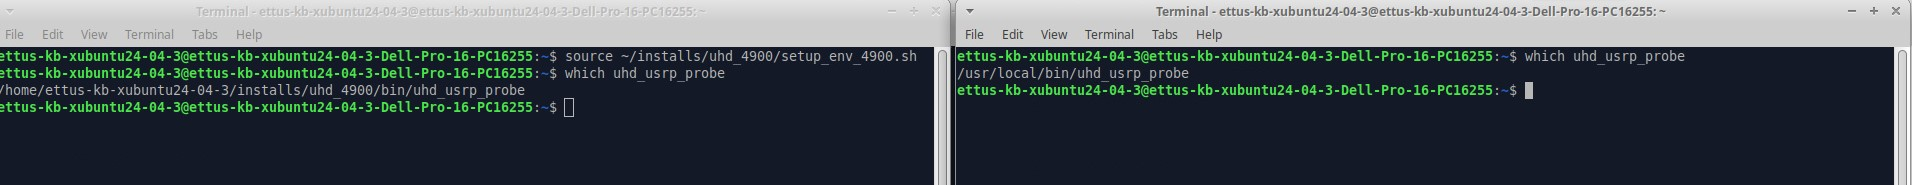
\includegraphics[width=0.85\linewidth]{latex/jpg_png/image_Comparison of 4.9.0.0 and 4.9.0.1.jpg}
\end{center}

\vspace{0.2cm}

\begin{itemize}
    \item \textbf{\textcolor{DarkBlue}{Step 9: Load the UHD 4.9.0.0 FPGA Image onto the USRP}}
\end{itemize}

\scriptsize

\hspace*{2.8em}
\parbox{0.9\linewidth}{\scriptsize
In this example, the FPGA image corresponding to the locally installed
\textbf{UHD 4.9.0.0} is loaded onto the USRP instead of the FPGA image from the
system-wide UHD installation. This demonstrates that when multiple UHD versions
are installed, each version can use its own compatible FPGA images for testing
and development without affecting the primary installation.
}

\vspace{0.2cm}

\begin{center}
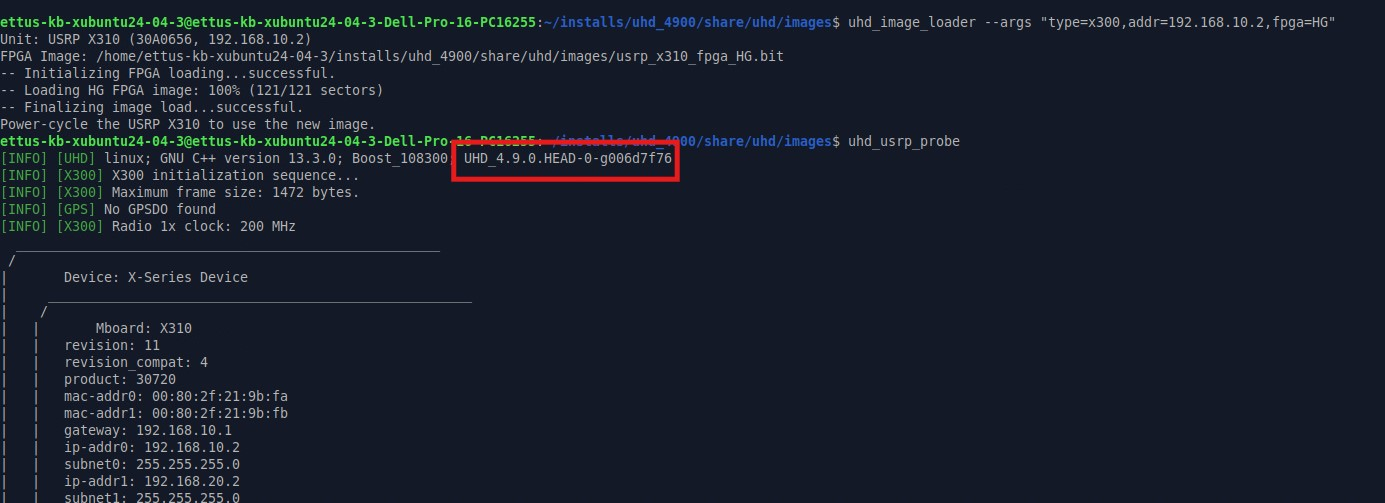
\includegraphics[width=0.53\linewidth]{latex/jpg_png/image_after loading 4.9.0.0 image on X310.jpg}
\end{center}

\end{frame}